
\chapter{Econometria Clássica e Efeitos Marginais}

Introduzido o conceito de Floresta Aleatória, agora voltamos nossa atenção à Econometria Clássica e seu \textit{workhorse model}, o \textbf{modelo clássico de regressão linear}. Veremos uma maneira de estimar os parâmetros desse modelo, via Mínimos Quadrados Ordinários, como modelos de Floresta Aleatória não têm a mesma interpretabilidade e como podemos contornar essa problemática avaliando o modelo na vizinhança de algumas observações. 



\section{Teoria Clássica de Regressão Linear}

Recuperando o conceito apresentado no início do capítulo interior, um \textbf{modelo} é um mapa entre um espaço de mensuração $\X$ (que neste contexto tem seus elementos chamados de \textbf{variáveis independentes}), com variáveis ditas explicativas do fenômeno representado no espaço de resposta $\Y$. \citeonline{hayashi} descreve modelos, em um linguajar mais estatístico como (i) um conjunto de restrições sobre a distribuição conjunta das variáveis e/ou (ii) um conjunto de distribuições conjuntas satisfazendo um conjunto de hipóteses. Iremos nos referir às variáveis medidas em $\X$ como \textbf{regressores}. Nesta seção iremos descrever uma família de modelos lineares, suas limitações e virtudes.



\begin{hipotese}[Linearidade]
Nossos modelos $\mathcal{L} : \X \to \Y$ são funções lineares. Nos referimos ao valor da $i$-ésima observação na $j$-ésima variável como $x_{ij}$, sua resposta sendo $y_i$. O termo $\epsilon_i$ é o \textbf{resíduo}, uma variável aleatória que acomodará a parcela não-explicada pelas variáveis em $\X$ da resposta em $\Y$. Se $\X \subset \R^k$ então o vetor de parâmetros que estimaremos será $\boldsymbol{\beta} \in \R^k$ e nossos modelos terão a forma funcional:

\begin{align}
    y_i = \sum_{j = 1}^k \beta_j x_{ij} + \epsilon_i \label{mod_lin}
\end{align}

Linearidade implica que o efeito de uma variação em um regressor particular na resposta não depende do seu nível, nem do de outros regressores. De fato:

\begin{align}
    \frac{\partial y}{\partial x_i} = \beta_i
\end{align}
\end{hipotese}


Essa hipótese pode parecer muito restritiva a princípio, mas não é (tanto assim). O modelador pode usar de intuição para construir variáveis novas que são funções não-lineares das variáveis mensuradas originalmente. A relação entre salário e experiência ou escolaridade, por exemplo, tem retornos decrescentes. Os primeiros cinco anos no mercado de trabalho contribuem muito mais para um aumento salarial do que os últimos cinco anos de carreira. Essa relação pode ser captada introduzindo um termo com o quadrado da experiência no modelo ou uma variável discreta valendo $1$ nos primeiros anos de carreira e $0$ depois, por exemplo. 

\begin{exemplo}[Estimando linearmente uma relação não-linear]

Suponha que algum processo de interesse dependa de uma variável aleatória $x$ com a seguinte relação: $y(x) = 100 + 2x - 5x^2$. Observamos $y$ com um erro:

\begin{figure}[H]
    \centering
    
    \captionbox{Uma amostra simulada do processo. Elaboração própria.}{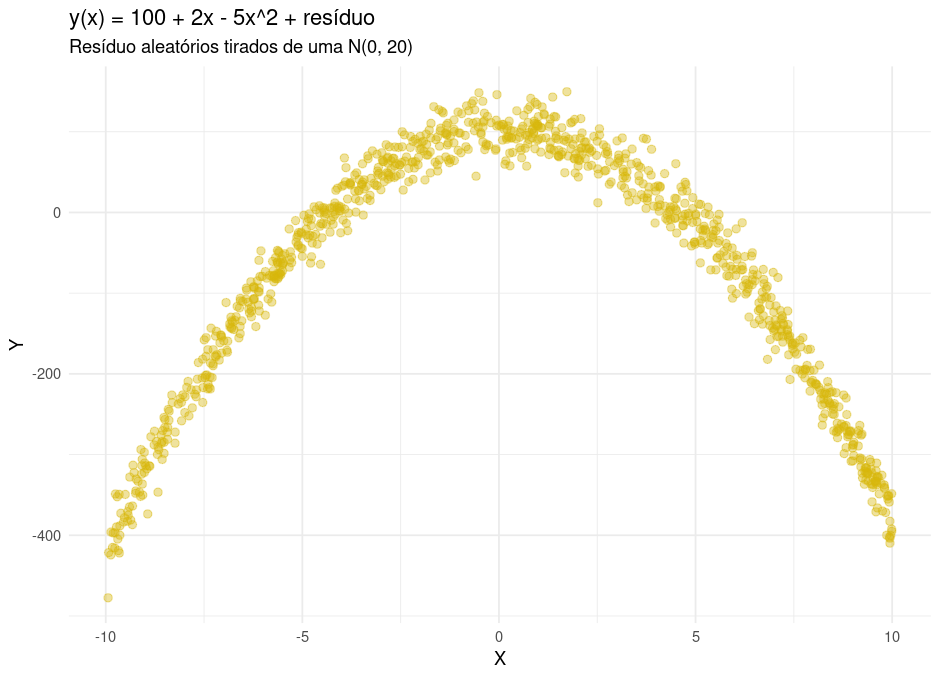
\includegraphics[scale = .75]{imagens/exemplo4_dist.png}}
\end{figure}

As tabelas \ref{tab:tabela1_exemplo4} e \ref{tab:tabela2_exemplo4} mostram as estimativas de dois modelos, um com $x$ e uma constante, outro com $x$, a constante e $x^2$. O segundo modelo recupera os parâmetros com erros da ordem de $1\%$, o primeiro errou por alguns desvios-padrão tanto a inclinação quanto o intercepto. 

\begin{table}

\caption{\label{tab:tabela1_exemplo4}Modelo sem termo quadrático}
\centering
\begin{tabular}[t]{l|r|r|r|r}
\hline
termo & estimativa & erro\_padrao & estatistica\_t & p\_valor\\
\hline
(Intercept) & 35.454087 & 1.9612419 & 18.07737 & 0\\
\hline
x & 5.158627 & 0.3444152 & 14.97793 & 0\\
\hline
\end{tabular}
\end{table}

\begin{table}

\caption{\label{tab:tabela2_exemplo4}Modelo com termo quadrático}
\centering
\begin{tabular}[t]{l|r|r|r|r}
\hline
term & estimate & std.error & statistic & p.value\\
\hline
(Intercept) & 100.169896 & 0.9422816 & 106.30569 & 0\\
\hline
x & 4.997511 & 0.1111325 & 44.96895 & 0\\
\hline
x2 & -1.996669 & 0.0215421 & -92.68662 & 0\\
\hline
\end{tabular}
\end{table}


A introdução de novas variáveis, funções não-lineares das originais, expande o número de situações em que a aproximação linear não é uma simplificação exagerada da realidade. Isso ocorre, inclusive, sem perda de interpretabilidade. Para entender o efeito marginal de uma variável que tenha sido ''expandida'' com transformações não-lineares basta somar as derivadas da resposta em relação à original bem como às expansões.


\end{exemplo}

Antes de prosseguir é importante apresentar a notação matricial dos modelos lineares. Uma maneira interessante de nos referir aos dados coletados de uma amostra - e como discutiremos estimação isso é importante - é associa-los à uma matriz. Notaremos uma \textbf{matriz de dados} como $\mathbf{X}$ em que $\mathbf{X}_{ij}$ é a medida da $i$-ésima observação na $j$-ésima variável. Também teremos $\mathbf{y}$, o vetor em que a $i$-ésima entrada é a medida da variável resposta da $i$-ésima observação, e $\mathbf{\epsilon}$, o vetor com o resíduo. A partir de agora usaremos $n$ para nos referir ao tamanho da amostra, o número de linhas em $\mathbf{X}$ e $\mathbf{y}$. Reescrevendo a equação \ref{mod_lin} em notação matricial:

\begin{equation}
    \underset{n \times 1}{\mathbf{y}} = \underset{n \times k}{\mathbf{X}} \,\, \underset{k \times 1}{\boldsymbol{\beta}}   + \underset{n \times 1}{\boldsymbol{\epsilon}}
\end{equation}



\begin{hipotese}[Exogeneidade Estrita]
A média condicional do resíduo é nula.

\begin{align}
    \E[\epsilon_i \, | \, \mathbf{X}] = 0
\end{align}

Enquanto função dos dados, a média condicional dos resíduos não necessariamente é linear. Podemos nos livrar desse problema supondo que, no entanto, assume o valor constante de zero. Essa hipótese não é restritiva se, entre as variáveis explicativas, houver uma com valor constante igual à média incondicional dos resíduos. É assim de trás para frente que encontraremos o valor constante do modelo no processo de estimação, inclusive. 

\end{hipotese}

\begin{hipotese}[Ausência de Multicolinearidade]
O posto da matriz de dados $\mathbf{X}_{n \times k}$ é $k$ com probabilidade 1.
\end{hipotese}

Em termos práticos, supomos que as variáveis dadas para um modelo linear são linearmente independentes umas das outras. Se os valores de uma variável podem ser inteiramente determinados por combinações lineares de outras, qualquer informação que possa trazer já está contida nas outras.

Também supomos que nosso modelo erra de maneira consistente:

\begin{hipotese}[Homocedasticidade]
A variância dos erros independe do nível dos regressores:

\begin{align}
    \E[\epsilon_i^2\, |\, \mathbf{X} ] = \sigma^2
\end{align}


\end{hipotese}

\begin{exemplo}[Heterocedasticidade]
É fácil quebrar o exemplo anterior, basta tornar o componente não-observado uma função de alguma variável explicativa. Adicionando esse comportamento no processo simulado temos:

\begin{figure}[H]
    \centering
    
    \captionbox{Uma amostra simulada do processo. Elaboração própria.}{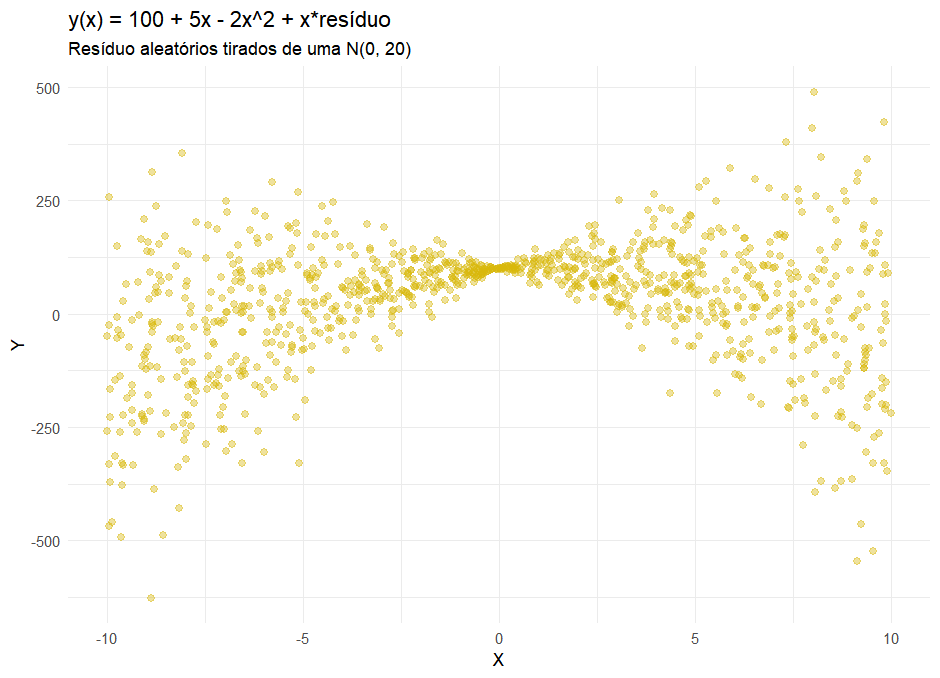
\includegraphics[scale = .75]{imagens/exemplo_heteroske.png}}
\end{figure}

\begin{table}

\caption{\label{tab:tabela_hetero}Modelo com termo quadrático. Elaboração própria.}
\centering
\begin{tabular}[t]{l|r|r|r}
\hline
termo & estimativa & erro\_padrao & estatistica\_t\\
\hline
(Intercept) & 97.64 & 6.97 & 14.01\\
\hline
x & 24.72 & 3.15 & 7.86\\
\hline
x2 & -2.37 & 0.30 & -7.95\\
\hline
\end{tabular}
\end{table}


Agora quando tentamos recuperar os parâmetros obtemos estimativas estatisticamente significantes, como informa a tabela \ref{tab:tabela_hetero}. Os parâmetros estimados, no entanto, estão à dezenas de desvios-padrão dos verdadeiros.


\end{exemplo}



% Dadas as Condições de Gauss-Markov e uma amostra $(\mathbf{X}, \mathbf{y})$, se $(\mathbf{x}_i, \mathbf{y}_i)$ são i.i.d vale que $ \E[\epsilon_i^2\, |\, \mathbf{X} ] = \E[\epsilon_i^2\, |\, \mathbf{x}_i ]  $.


\section{Efeitos Marginais}
\subsection{Em Modelos Lineares}
A primeira hipótese, Linearidade, é a chave aqui. A resposta, supomos, varia linearmente nos regressores. Podemos introduzir algumas interações criando variáveis novas que são funções não-lineares das variáveis originais, adicionamos logaritmos, potências, indicadoras e outras tantas transformações para acomodar não-linearidades. Essa abordagem promissora, no entanto, quebra rapidamente sob presença de heterocedasticidade. Mesmo que não haja heterocedasticidade, adicionar regressores diminui a precisão da estimativa.

E mesmo sob as condições que descrevemos, identificamos a média dos modelos marginais. Podemos falar com alguma confiança de elasticidades, semi-elasticidades, mas serão sempre aproximações para o suporte inteiro da variável. Nem todos os efeitos marginais nasceram iguais e não é crível que sejam constantes em todo o espaço de mensuração $\X$. Uma maneira de contornar o problema é regressão quantílica, que vem ao custo de cada fatia no domínio diminuir a amostra que cada modelo poderá receber.





Com florestas aleatórias nenhum dos dois problemas anteriores está presente. Podemos até realizar inferência ao usar vários modelos diferentes para construir uma distribuição de efeitos marginais. 

\subsection{Em Florestas Aleatórias}

Suponha que temos uma árvore treinada $\A$ e uma observação $x$. Com alguma licença poética nos referimos à previsão dessa árvore para essa obervação como $\A(x)$. De maior incômodo para o econometrista é que não é claro o que exatamente é a derivada dessa função. Isso é um problema porque boa parte da utilidade de um modelo (linear) estimado é ter um vetor de parâmetros intuitivamente interpretáveis, pois contém as derivadas parciais do modelo. 

A derivada de $\A(\cdot)$, seja lá como for, não é tão informativa. Uma pertubação em uma observação $x$ só altera o resultado da previsão de uma árvore se for grande o suficiente para deslocar $x$ para outra regra de classificação/previsão. Teríamos uma função que é nula em boa parte de seu domínio, descontínua onde não for. 

O problema é atenuado com uma floresta aleatória. Uma pertubação pequena em $x$ pode alterar a previsão de uma fração das árvores da florestas. Com um número suficientemente grande de árvores uma variação arbitrariamente pequena em $x$ leva à uma variação arbitrariamente pequena em $\F(x)$ e vale alguma forma de continuidade. 

Esse caminho sugere uma estratégia promissora. Podemos perturbar uma observação de referência e as previsões de seus vizinhos. Isso gera uma curva relacionando valores de um regressor, dado um vetor níveis para os outros regressores, às previsões. Sua inclinação nos dá os efeitos marginais, que ao contrário do que acontece em modelos lineares, são sensíveis aos níveis dos regressores que não estamos perturbando.

\section{Um Procedimento de Computação}

Suponha um modelo $\M : \X \to \Y$. Como computamos seus efeitos marginais de maneira agnóstica? Gostaríamos de aplicar um mesmo procedimento e identificar os efeitos marginais sem depender da mecânica particular de uma classe de modelos. Por trás dos panos cada classe opera um maquinário completamente diferente: redes neurais são composições sucessivas de transformações lineares, modelos lineares são polinômios, máquinas de vetores de suporte calculam distâncias de vetores a um hiperplano estimado com base nos dados. 

Se as mecânicas internas de $\M$ variam demais para termos um procedimento uniforme, podemos olhar onde não há variação entre classes de modelos, $\X$ e $\Y$. Observando os valores que as predições do modelo dão para a resposta $Y$ em uma curva parametrizada $t \in \X$ basta computar a sua derivada (e isso sabemos fazer!) para achar os efeitos marginais na curva. 

Como normalmente estamos interessados no efeito de tratamento individual de uma variável, talvez seu efeito conjunto com outra, o problema é limitado a avaliar o modelo ao longo de uma ou duas dimensões apenas. Avaliar o efeito marginal de mais variáveis implica apenas repetir o procedimento, não sofrer da maldição da dimensionalidade. Esse procedimento é computacionalmente simples, barato e agnóstico ao modelo.
